\scanpage{12}
\mspage{10}

qu'i\unsure{\deleted{m}l|\deleted{o}l|\deleted{l}m|\deleted{l}o} conviendra de poser les définitions adéquates). - Peut-être Quill
\margin{\handwritten{\uuline{\unsure{oui|sic}}}\figure{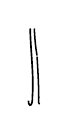
\begin{tikzpicture}[x=.035cm,y=.035cm,baseline=0pt]\draw[line width=.6pt] (0,27)..controls(.15,19)and(1.4,10)..(.8,2)..controls(.9,.4)and(.5,-1)..(-.1,-.8)..controls(-.6,-.6)and(-.6,.1)..(-.6,.8);\draw[line width=.55pt] (1.5,27)..controls(1.8,21)and(2.2,19)..(2.5,17.2);\draw[line width=.55pt] (2.5,16.8)..controls(2.8,12)and(3.2,5)..(3.1,.1)--(3.4,-.5);\end{tikzpicture}}}a-t-il une définition semi-simpliciale plus directe, sans passer par des
n-catégories, des $K_i$ et plus précisément du H-espace qui devrait correspo
dre à C. \deleted{Dans le cas} Ce n'est certainement \unsure{pas \inserted{en général} l'ensemble|\inserted{en général} pas l'ensemble} semi-simplicial
SC \deleted{engendré à} associé à C, puisque dans le cas d'une catégorie additive,
C est homotopiquement trivial (en effet le foncteur identique est ``homoto
au foncteur nul, puisqu'il suffit d'avoir un homomorphisme d'un foncteur
dans l'autre; d'où une équivalence d'homotopie entre C et la catégorie
nulle). Pourtant, il semble bien que dans le cas où C est une Gr-catégor
\margin{\figure{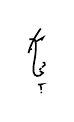
\begin{tikzpicture}[x=.04cm,y=.04cm,baseline=0pt]\draw[line width=.6pt] (1.1,11)..controls(1.7,13.8)and(3.5,16.7)..(5.0,18.8);\draw[line width=.6pt] (1.4,15.4)--(3.0,15.4)..controls(3.5,14.7)and(3.5,13.5)..(3.4,12.2)..controls(3.4,9.6)and(2.4,6.9)..(2.7,5.0)..controls(2.9,3.6)and(4.4,3.1)..(5.7,4.7)--(4.7,5.3);\draw[line width=.55pt] (3.2,14.5)--(5.8,16.0)--(5.2,15.0);\draw[line width=.5pt] (1.3,12.0)--(2.2,12.3);\draw[line width=.55pt] (5.6,8.0)--(6.2,8.0)--(6.3,7.2)--(5.4,6.5);\draw[line width=.55pt] (5.2,6.2)--(4.5,5.7);\draw[line width=.55pt] (4.1,1.0)--(5.3,1.1)--(4.8,.9)..controls(4.9,.3)and(5.4,-.1)..(5.1,-.8);\draw[line width=.7pt,line cap=round] (5.15,-1.5)--(5.18,-1.55);\end{tikzpicture}}\figure{\begin{tikzpicture}[x=.04cm,y=.04cm,baseline=0pt]\draw[line width=.6pt] (0,25)--(.7,24.9)..controls(1.1,24.7)and(.1,23.0)..(.2,22.0)..controls(.2,21.4)and(1.1,21.0)..(1.1,20.3)--(1.2,17.9);\draw[line width=.6pt] (1.2,17.2)--(1.3,16.3);\draw[line width=.3pt,opacity=.4] (1.35,15.3)--(1.4,15.0);\draw[line width=.3pt,opacity=.4,line cap=round] (1.5,12.7)--(1.5,12.6);\draw[line width=.4pt,line cap=round] (1.8,9.0)--(1.8,8.8);\draw[line width=.55pt] (2.1,6.6)--(2.2,6.2);\draw[line width=.3pt,opacity=.4] (2.5,4.0)--(2.5,3.7);\draw[line width=.6pt,line cap=round] (2.2,.2)--(2.3,.15);\end{tikzpicture}}}i.e. admet des inverses, alors ce soit bien la construction ``naïve'' SC qu
est la bonne, puisqu'on trouve bien un $\handwritten{\pi}_o$ et un $\handwritten{\pi}_1$ qui sont aussi les
$\handwritten{\pi}_o$ et $\handwritten{\pi}_1$ au sens catégorie sans Gr-structure.

\handwritten{À expliquer : pour des Gr-n-catégories, les $\pi_i$ au sens}
\margin{\figure{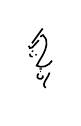
\begin{tikzpicture}[x=.04cm,y=.04cm,baseline=0pt]\draw[line width=.6pt] (1.2,17.3)--(4.6,22.0);\draw[line width=.6pt] (.2,16.5)..controls(.1,15.6)and(.8,15.6)..(1.3,16.0)--(3.4,18.3);\draw[line width=.6pt] (3.8,19.4)--(4.7,19.9)..controls(5.6,19.3)and(5.8,18.4)..(5.8,17.0)..controls(5.5,14.2)and(3.6,12.2)..(2.7,10.2)..controls(4.2,9.3)and(6.5,10.0)..(7.6,11.8);\draw[line width=.55pt,line cap=round] (1.3,14.7)--(1.5,14.9);\draw[line width=.55pt] (.5,14.0)..controls(.3,13.3)and(.8,13.1)..(1.4,13.0);\draw[line width=.5pt] (2.3,13.5)--(2.7,13.8);\draw[line width=.5pt] (3.6,9.1)--(4.3,9.2);\draw[line width=.6pt] (3.3,7.7)..controls(2.5,6.7)and(2.9,5.9)..(4.1,6.0)..controls(4.8,6.1)and(4.7,6.7)..(4.6,7.1);\draw[line width=.6pt] (6.8,8.0)..controls(6.4,6.6)and(5.1,5.3)..(5.0,4.3)..controls(4.9,3.8)and(5.2,3.4)..(5.6,3.2);\draw[line width=.35pt] (3.8,8.2)--(4.0,8.5);\end{tikzpicture}}\figure{\begin{tikzpicture}[x=.03cm,y=.03cm,baseline=0pt]\draw[line width=.6pt] (.7,34.5)--(.8,34.1);\draw[line width=.45pt] (.8,33.3)--(.8,32.9);\draw[line width=.35pt] (.7,32.4)--(.7,32.1);\draw[line width=.45pt] (.6,31.6)--(.3,30.7);\draw[line width=.6pt] (.2,24.9)--(.2,24.2);\draw[line width=.6pt] (.2,23.8)..controls(.2,21.2)and(.1,19.1)..(.3,17.8);\draw[line width=.6pt] (.2,16.3)--(.2,15.5);\draw[line width=.45pt] (.2,15.1)--(.2,14.6);\draw[line width=.45pt] (.2,14.2)--(.2,13.8);\draw[line width=.55pt,line cap=round] (.2,13.0)--(.2,12.8);\draw[line width=.6pt] (-.1,9.0)..controls(.0,6.7)and(.5,4.2)..(.5,1.8);\draw[line width=.65pt,line cap=round] (.4,.9)--(.5,.8);\end{tikzpicture}}}\handwritten{semi-simplicial sont aussi les $\pi_i$ au sens Gr-n-catégories,}
\handwritten{savoir les objets à isom près dans divers \uline{Hom}$(1,1)$\,..... . \deleted{Il y a
aussi une interprétation de l'opération $\Omega$ : \unsure{esp} des lacets
en termes d'opération du shift géométrique évidente sur les
n-catégories.....}}

\margin{11}
